\newcommand{\standalone}{}
\documentclass[a4paper,11pt,oneside]{book}

%%% το αρχείο αυτό καθορίζει το look που έχουν οι pythonies
%%% γίνεται \input από όλα τα κεφάλαια και τα φύλλα εργασίας

% χρησιμοποιούμενα πακέτα: 
% 
% polyglossia
% xstring
% graphicx
% caption
% xcolor
% hyperref
% minted
% geometry
% titlesec
% datetime
% changepage
% ntheorem

% οριζόμενες εντολές:
%
% smallcaps (βοηθ. removeaccents)
%    μικρά κεφαλαία χωρίς τόνους στα φωνήεντα
% scaling
%    η κλιμάκωση *όλων* των illustrations, τρέχουσα τιμή 0.9
% iconcomputer, iconkeyboard, icondiscuss, iconfillin, iconcaution, iconprompt, dottedline
%    εικονίδια για τα φύλλα εργασίας και εστιγμένη γραμμή
% marginnote
%    πλευρικό σχόλιο
% chapterwabstract (βοηθ. abstract, boxcolor, chaptercolor, concepts, tmpconcepts)
%    εισαγωγικό κείμενο κεφαλαίου με χρωματιστό τετράγωνο, συνοδευτικές έννοιες, κλπ.
% tobecontinued
%    εμφανίζει το "συνεχίζεται στην επόμενη σελίδα"

% οριζόμενα περιβάλλοντα:
% 
% note
%    μια υποσημείωση ή υπόδειξη, με μικρότερα γράμματα
% question
%    μια ερώτηση που "οδηγεί" κάθε νέα ενότητα
% answer
%    μια απάντηση σε μια ερώτηση του φύλλου εργασίας
% theory
%    μια ενότητα "θεωρίας" (στο τέλος ενός κεφαλαίου)
% exercise
%    μια αριθμημένη άσκηση
% step
%    ένα αριθμημένο βήμα (για φύλλο εργασίας)

% για μορφοποίηση κώδικα:
%
% pycode (περιβάλλον)
%     κώδικας python χωρίς αρίθμηση
% pyfile (εντολή)
%     εισαγωγή κώδικα python από αρχείο
% pyfilenl (εντολή)
%     εισαγωγή κώδικα python από αρχείο χωρίς αρίθμηση γραμμών
% pyfilesrc (εντολή)
%    εισαγωγή κώδικα από αρχείο με link στο αρχείο
% pyinline (εντολή)
%     κώδικας python μέσα στη ροή του κειμένου
% pyplain (περιβάλλον, για τα φύλλα εργασίας)
%     κώδικας python χωρίς φόντο
% pynew (περιβάλλον, για τα φύλλα εργασίας)
%     κώδικας python με φόντο
% pyterm (περιβάλλον για τα φύλλα εργασίας)
%     η είσοδος του χρήστη ή τα περιεχόμενα της οθόνης
% pyhighlight (εντολή)
%    highlight κειμένου (χρησιμοποιείται για κώδικα μέσα σε pyplain)


%%% επιλογές γλώσσας και γραμματοσειρών για το XeLaTeX

\usepackage{polyglossia}
\setdefaultlanguage{greek}
\setmainfont[Ligatures=TeX,SmallCapsFont={Linux Libertine O C},SmallCapsFeatures={Letters=SmallCaps}]{Linux Libertine O}
\setsansfont{Linux Biolinum O}
\setmonofont{Ubuntu Mono}
\enablehyphenation

% αφαίρεση τόνων από τα smallcaps
\usepackage{xstring}
\newcommand{\removeaccents}[1]{%
\def\result{#1}%
\StrSubstitute{\result}{ά}{α}[\result]%
\StrSubstitute{\result}{έ}{ε}[\result]%
\StrSubstitute{\result}{ή}{η}[\result]%
\StrSubstitute{\result}{ί}{ι}[\result]%
\StrSubstitute{\result}{ό}{ο}[\result]%
\StrSubstitute{\result}{ύ}{υ}[\result]%
\StrSubstitute{\result}{ώ}{ω}[\result]%
\StrSubstitute{\result}{Ά}{Α}[\result]%
\StrSubstitute{\result}{Έ}{Ε}[\result]%
\StrSubstitute{\result}{Ή}{Η}[\result]%
\StrSubstitute{\result}{Ί}{Ι}[\result]%
\StrSubstitute{\result}{Ό}{Ο}[\result]%
\StrSubstitute{\result}{Ύ}{Υ}[\result]%
\StrSubstitute{\result}{Ώ}{Ω}[\result]%
\result
}

\newcommand{\smallcaps}[1]{\textsc{\removeaccents{#1}}}

%%% εικόνες και λεζάντες

\usepackage{graphicx}
\newcommand{\scaling}{0.9}
\usepackage{caption}
\captionsetup{font=footnotesize}

%%% ειδικά περιβάλλοντα

\usepackage{xcolor}

% ερωτήσεις (που οδηγούν στην επόμενη ενότητα)
\definecolor{questioncolor}{rgb}{0.6,0.5,0.5}
\newenvironment{question}{\noindent\itshape\color{questioncolor}}{\noindent\ignorespaces}

% απαντήσεις (για τις ερωτήσεις των φύλλων εργασίας)
\definecolor{answercolor}{rgb}{0.5,0.5,0.5}
\newenvironment{answer}{\marginnote[16pt]{\iconfillin}\noindent\itshape\color{answercolor}}{\noindent\ignorespaces}

% περιβάλλον "θεωρίας" (πλήρες πλάτος κειμένου)
\usepackage{changepage}
\newenvironment{theory}[1]{\begin{adjustwidth}{}{-\overhang}\smallcaps{#1}\itshape}{\end{adjustwidth}}

% απομεινάρια...
% \newlength{\theoryrulelength}
% \setlength{\theoryrulelength}{36pt}
% \newenvironment{theory}{\rule{\theoryrulelength}{0.4pt}\begin{adjustwidth}{}{-\overhang}\itshape}{\end{adjustwidth}\rule{\theoryrulelength}{0.4pt}}

%%% υπερσύνδεσμοι

\definecolor{linkcolor}{rgb}{0.0,0.5,0.25}
\usepackage[colorlinks=true,urlcolor=linkcolor]{hyperref}

%%% εικονίδια και εστιγμένες γραμμές (για τα φύλλα εργασίας)

\newcommand{\iconcomputer}{
\includegraphics[scale=0.35]{../../share/circle-icons/one-color/computer.eps}}
\newcommand{\iconkeyboard}{
\includegraphics[scale=0.35]{../../share/circle-icons/one-color/keyboard.eps}}
\newcommand{\icondiscuss}{
\includegraphics[scale=0.35]{../../share/circle-icons/one-color/chat.eps}}
\newcommand{\iconfillin}{
\includegraphics[scale=0.35]{../../share/circle-icons/one-color/compose.eps}}
\newcommand{\iconcaution}{
\includegraphics[scale=0.35]{../../share/circle-icons/one-color/caution.eps}}
\newcommand{\iconprompt}{
\includegraphics[scale=0.35]{../../share/circle-icons/one-color/prompt.eps}}
\newcommand{\dottedline}{\vspace{\parskip}\dotfill}

%%% συνεχίζεται στην επόμενη σελίδα

\newcommand{\tobecontinued}{\mbox{}\hfill{\footnotesize ...συνεχίζεται στην επόμενη σελίδα.}}
\newenvironment{note}{\small\upshape}{}

%%% μορφοποίηση κώδικα με το pygmentize

\usepackage{minted}

% fix για ένα bug στο minted που εμφανίζεται όταν χρησιμοποιείται χρώμα στο φόντο (bgcolor)
% http://tex.stackexchange.com/questions/228058/how-to-space-before-and-after-a-minted-code-block-with-bgcolor
\makeatletter
\patchcmd{\minted@colorbg}{\noindent}{\noindent}{}{}
\apptocmd{\endminted@colorbg}{}{}{}
\makeatother

% χρώματα φόντου για τον κώδικα
\definecolor{codebg}{rgb}{0.80,0.95,0.85}
\definecolor{newcodebg}{rgb}{0.75,0.95,0.85}

% ορισμοί για τα περιβάλλοντα κώδικα
% pycode: περιβάλλον κώδικα python χωρίς αρίθμηση
\newminted[pycode]{python3}{bgcolor=codebg}
% pyfile: python από αρχείο
\newmintedfile[pyfile]{python3}{linenos=true,numberblanklines=false,escapeinside=||,bgcolor=codebg}
% pyfilenl: python από αρχείο χωρίς αρίθμηση γραμμών
\newmintedfile[pyfilenl]{python3}{linenos=false,numberblanklines=false,escapeinside=||,bgcolor=codebg}
% pyinline: python μέσα στη ροή του κειμένου
\newmintinline[pyinline]{python3}{linenos=true,numberblanklines=false}
% pyplain: (για τα φύλλα εργασίας) περιβάλλον χωρίς φόντο
\newminted[pyplain]{python3}{bgcolor=white,escapeinside=||,formatcom={\upshape}}
% pynew: (για τα φύλλα εργασίας) περιβάλλον με φόντο
\newminted[pynew]{python3}{bgcolor=newcodebg,escapeinside=||,formatcom={\upshape}}
% pyterm: (για τα φύλλα εργασίας) περιβάλλον για τα περιεχόμενα της οθόνης
\newminted[pyterm]{text}{bgcolor=white,escapeinside=||}

%\newminted[pyterm]{text}{escapeinside=||}
% [TODO] fix: το pyterm χωρίς bgcolor εμφανίζει μεγαλύτερα περιθώρια (πάνω και κάτω) και δεν φαίνεται ωραίο. Το bgcolor είναι προσωρινό workaround, έχει κι αυτό margins (για να μην είναι κολλητά ο κώδικας με το περιθώριο) κι έτσι ο κώδικας στ' αριστερά δεν είναι τέλεια στοιχισμένος.

% εντολή για κώδικα από αρχείο με link στο αρχείο
\newcommand{\pyfilesrc}[2][]{%
\pyfile[#1]{#2}\\
\mbox{}\hfill{\scriptsize\href{http://pythonies.mysch.gr/#2}{\url{#2}}}
}

% εντολή για το highlighting του κώδικα (συνήθως σε pyplain περιβάλλον με escapeinside)
\newcommand{\pyhighlight}[1]{\colorbox{newcodebg}{#1}}

%%% αριθμημένα περιβάλλοντα

\usepackage{ntheorem}

% άσκηση
\makeatletter
\theoremheaderfont{\upshape}%\upshape\bfseries\scshape}
\theorembodyfont{\itshape}%\slshape}
\newtheoremstyle{lmargin}%
  {\item[\theorem@headerfont \llap{##2}\hskip\labelsep\hskip-6pt]}%
  {\item[\theorem@headerfont \llap{##2}\hskip\labelsep ##1\ (##3)\theorem@separator]}
\makeatother
\theoremstyle{lmargin}
\newtheorem{exercise}{}[chapter]

% βήμα φύλλου εργασίας
\makeatletter
\theoremheaderfont{\bfseries}%\upshape\bfseries\scshape}
\theorembodyfont{\upshape}%\slshape}
\newtheoremstyle{lmarginup}%
  {\item[\theorem@headerfont \llap{##2}\hskip\labelsep\hskip-6pt]}%
  {\item[\theorem@headerfont \llap{##2}\hskip\labelsep ##1\ (##3)\theorem@separator]}
\newtheoremstyle{slmarginup}%
  {\item[\theorem@headerfont \llap{##1##2.}\hskip\labelsep\hskip-6pt]}%
  {\item[\theorem@headerfont \llap{##2.}\hskip\labelsep ##1\ (##3)\theorem@separator]}
\makeatother

% deprecated: \newcommand{\standalone}{} to define standalone
%\ifdefined\standalone
    \theoremstyle{slmarginup}
    \newtheorem{step}{}
%\else
%    \theoremstyle{lmarginup}
%    \newtheorem{step}{}[chapter]
%\fi

%%% γεωμετρία σελίδας και συναφείς ορισμοί από το tufte-latex
%%% https://tufte-latex.github.io/tufte-latex/

% εσοχή και διάστημα μεταξύ παραγράφων
% δεν επηρρεάζει το tufte-latex
\parindent=0pt
\parskip=6pt

% γεωμετρία σελίδας και ορισμός μηκών
\usepackage[a4paper,left=24.8mm,top=27.4mm,headsep=2\baselineskip,textwidth=107mm,marginparsep=8.2mm,marginparwidth=49.4mm,textheight=66\baselineskip,headheight=\baselineskip]{geometry}

\setlength{\marginparpush}{12pt}
\addtolength{\marginparpush}{\parskip}
\newlength{\fullwidth}
\setlength{\fullwidth}{\textwidth}
\addtolength{\fullwidth}{\marginparsep}
\addtolength{\fullwidth}{\marginparwidth}
\newlength{\overhang}
\setlength{\overhang}{\marginparsep}
\addtolength{\overhang}{\marginparwidth}

% απομεινάρια...
%\setlength\abovedisplayskip{6pt plus 2pt minus 4pt}
%\setlength\belowdisplayskip{6pt plus 2pt minus 4pt}

% italicize description run-in headings (instead of the default bold)
\renewcommand*\descriptionlabel[1]{\hspace\labelsep\normalfont\em #1}

% πλευρική σημείωση
\newcommand\marginnote[2][0pt]{%
  \marginpar{\hbox{}\vspace*{#1}\vspace*{-1\baselineskip}\noindent \footnotesize\textup{#2}}%
  {}%
}

% formatting title sections
\setcounter{secnumdepth}{-1}

\usepackage{titlesec}
\usepackage[nodate]{datetime}
\newlength{\beforesection}
\setlength{\beforesection}{3ex plus 0.5ex minus 0.2ex}
\addtolength{\beforesection}{-\parskip}
\newlength{\aftersection}
\setlength{\aftersection}{1.5ex plus 0.2ex}
\addtolength{\aftersection}{-\parskip}
\titlespacing*{\section}{0pt}{\beforesection}{\aftersection}

% απομεινάρια...
%\titlespacing*{\chapter}{0pt}{50pt}{40pt}
%\titlespacing*{\section}{0pt}{3.5ex plus 1ex minus .2ex}{2.3ex plus .2ex}

%%% για εισαγωγικό κείμενο κεφαλαίου με χρωματιστό τετράγωνο, συνοδευτικές έννοιες, κλπ.

\newcommand{\abstract}{}
\newcommand{\boxcolor}{}
\newcommand{\chaptercolor}{}
\newcommand{\concepts}{}
\newcommand{\tmpconcepts}{}
\newif\ifbonus

% reference: \titleformat{ command }[ shape ]{ format }{ label }{ sep }{ before-code }[ after-code ]
\titleformat{\chapter}[block]
{\Huge\sffamily}
{}
{0pt}
{\ifbonus\marginnote[-6pt]{\fcolorbox{\boxcolor}{\chaptercolor}{\makebox(40,40){\strut\textcolor{\boxcolor}{\Huge\thechapter}}}\\\vspace{\parskip}\\\tiny\today\\ \currenttime}\else\marginnote[-6pt]{\colorbox{\boxcolor}{\makebox(40,40){\strut\textcolor{\chaptercolor}{\Huge\thechapter}}}\\\vspace{\parskip}\\\tiny\today\\ \currenttime}\fi}
[\small\rmfamily\textmd\abstract\vspace{\parskip}\concepts\vspace{\parskip}\\\mbox{}\hrulefill]

\newcommand{\chapterwabstract}[5]{
	\renewcommand{\abstract}{#2}
    \renewcommand{\tmpconcepts}{#3}
	\ifdefempty{\tmpconcepts}{\renewcommand{\concepts}{}}{\renewcommand{\concepts}{\\\textbf{Έννοιες: }\tmpconcepts}}
	\renewcommand{\boxcolor}{#4}
	\renewcommand{\chaptercolor}{#5}
	\chapter{#1}
}

\definecolor{introColor}{rgb}{0.25,0.5,0.75}
\definecolor{answerColor}{rgb}{0.25,0.75,0.5}
\definecolor{crapsColor}{rgb}{0.5,0.75,0.25}
\definecolor{subtractionColor}{rgb}{0.5,0.25,0.75}
\definecolor{guessColor}{rgb}{0.75,0.25,0.5}
\definecolor{nimColor}{rgb}{0.75,0.5,0.25}
\definecolor{planetColor}{rgb}{0.25,0.25,0.75}
\definecolor{hangmanColor}{rgb}{0.25,0.75,0.25}
\definecolor{oxoColor}{rgb}{0.75,0.25,0.25}

\setcounter{part}{1}
\setcounter{chapter}{2}

\usepackage{booktabs}

%%% DOCUMENT START

\begin{document}

\chapterwabstract{Mπαρμπούτι}{Σε πολλές αμερικάνικες ταινίες οι πρωταγωνιστές γίνονται εκατομμυριούχοι ή χάνουν τα πάντα παίζοντας ένα παιχνίδι με ζάρια, άγνωστο στους περισσότερους από μας. Η πλησιέστερη ελληνική εκδοχή του παιχνιδιού είναι το μπαρμπούτι, πηγή έμπνευσης για πολλούς άτυχους ρεμπέτες.

Ακολουθώντας τα βήματα του φύλλου εργασίας θ' αναπτύξουμε ένα πρόγραμμα με το οποίο ο χρήστης θα παίζει αυτό το παιχνίδι. Η υλοποίηση του παιχνιδιού θα γίνει σε στάδια, ξεκινώντας από απλούστερες εκδοχές του, μέχρι να φτάσουμε στην τελική, ολοκληρωμένη του μορφή. 
%Ακολουθώντας τα βήματα αυτού του φύλλου εργασίας, θα αναπτύξουμε ένα πρόγραμμα με το οποίο ο χρήστης θα παίζει αυτό το παιχνίδι, αφού όμως πρώτα περάσουμε από μερικά ενδιάμεσα, απλούστερα παιχνίδια.
}{δομή επιλογής, δομή επανάληψης, υποπρογράμματα}{crapsColor}{white}

%%%%%%%%

\marginnote[22pt]{%
Εισαγωγικό υλικό:\\
\href{http://pythonies.mysch.gr/chapters/answer.pdf}{\url{pythonies.mysch.gr/chapters/answer.pdf}}\\
\href{http://pythonies.mysch.gr/chapters/answer-worksheet.pdf}{\url{answer-worksheet.pdf}}\\
\href{http://pythonies.mysch.gr/chapters/guess-standalone.pdf}{\url{guess-standalone.pdf}}
}
Για ν' ακολουθήσετε αυτό το φύλλο εργασίας, θα πρέπει \emph{ήδη} να μπορείτε να κάνετε ένα πρόγραμμα να εμφανίζει μηνύματα, να διαβάζει τιμές και να επιλέγει την συμπεριφορά του ανάλογα με τις συνθήκες που επικρατούν κατά την εκτέλεσή του. Διαφορετικά, θα πρέπει πρώτα ν' ανατρέξετε στο \emph{εισαγωγικό υλικό}.

\marginnote[13pt]{%
Διαβάστε το αντίστοιχο κεφάλαιο:\\
\href{http://pythonies.mysch.gr/chapters/craps.pdf}{\url{pythonies.mysch.gr/chapters/craps.pdf}}
}
Σε αυτό το φύλλο θα εμβαθύνουμε στα παραπάνω και θα δούμε επίσης πως μπορούμε να κάνουμε τα προγράμματά μας να εκτελούν \emph{επαναληπτικά}, δηλαδή ξανά και ξανά, τις ίδιες εντολές.
Θα δούμε επίσης πως μπορούμε να φτιάχνουμε \emph{υποπρογράμματα}, δηλαδή ομάδες εντολών που υλοποιούν μια συγκεκριμένη λειτουργία και \emph{καλούνται} στα σημεία όπου θέλουμε να εκτελεστούν.

\section{Τυχαιότητα}

%Πολλές διαδικασίες, και ιδιαίτερα τα παιχνίδια, βασίζονται στην \emph{τυχαιότητα}. Γι' αυτό παίζουμε κορώνα--γράμματα, ρίχνουμε ζάρια ή ανακατεύουμε τα χαρτιά της τράπουλας. 

% [comment] Βασίλης: Γιατί; Μέχρι αυτό το σημείο δεν έχουν ιδέα τι πάνε να κάνουν ή πώς παίζεται το παιχνίδι. Ξαναβάλε την παράγραφο με τους κανόνες, όπως υπάρχει στο κεφάλαιο. [reply] Δεν θέλω να βάλω το πλήρες σύνολο των κανόνων στην αρχή γιατί μπορεί να μπερδέψει σε σχέση με τα απλούστερα ενδιάμεσα παιχνίδια που υλοποιούμε. Είναι όμως εύστοχη παρατήρηση ότι δεν υπάρχει πουθενά η γενική μορφή του παιχνιδιού, οπότε θα προσθέσω στο σημείο αυτό μια αδρή περιγραφή.

Στο παιχνίδι που θα υλοποιήσουμε, ο παίκτης ρίχνει δύο ζάρια. Το αποτέλεσμα του παιχνιδιού εξαρτάται από το \emph{άθροισμα} των ενδείξεων των δύο ζαριών: για κάποιες τιμές του αθροίσματος ο παίκτης κερδίζει, για κάποιες άλλες χάνει, ενώ υπάρχουν και περιπτώσεις που το αποτέλεσμα δεν κρίνεται από την πρώτη ζαριά.

Στην πραγματικότητα, κάθε φορά που ρίχνουμε ένα ζάρι παράγουμε έναν \emph{τυχαίο} αριθμό από το \pyinline{1} μέχρι και το \pyinline{6}. Οι βασικές εντολές της Python δεν μας παρέχουν κάποιο μηχανισμό για να μιμηθούμε αυτή τη διαδικασία.
\marginnote[17pt]{Οι βιβλιοθήκες είναι συλλογές από έτοιμα μικρά προγράμματα που μπορούμε να χρησιμοποιήσουμε στα προγράμματά μας.}
Για το σκοπό αυτό θα χρειαστεί να εισάγουμε στο πρόγραμμά μας μια από τις πολλές διαθέσιμες \emph{βιβλιοθήκες}, τη \pyinline{random}, η οποία παρέχει τη λειτουργικότητα που μας χρειάζεται.

\clearpage
\begin{step}
\emph{Ξεκινήστε} το πρόγραμμα σας με την εντολή που ακολουθεί, για να \emph{εισάγετε} τη βιβλιοθήκη \pyinline{random}:

\begin{pynew}
import random
\end{pynew}

\emph{Προσθέστε} τώρα την εντολή:

\begin{pynew}
dice1 = random.randint(1,6)
\end{pynew}

Στην εντολή αυτή χρησιμοποιείται η \emph{συνάρτηση} \pyinline{randint}, από τη βιβλιοθήκη \pyinline{random}.
Όταν εκτελεστεί το πρόγραμμα, θα παραχθεί μια τυχαία τιμή από το \pyinline{1} μέχρι και το \pyinline{6} και αυτή θα είναι η τιμή της μεταβλητής \pyinline{dice1}.

% [comment] Πιθανές ερωτήσεις: Τί πιστεύετε ότι θα συμβεί αν αντί για 1 και 6 βάλουμε τις τιμές 100 και 1000; Τί τιμές πρέπει να χρησιμοποιήσουμε αντί για τις 1 και 6, ώστε να παίξουμε κορώνα--γράμματα;
\end{step}

\begin{step}
Τώρα \emph{προσθέστε} ακόμα μια εντολή που παράγει με τον ίδιο τρόπο την ένδειξη του δεύτερου ζαριού και την ονομάζει \pyinline{dice2}.
\end{step}

\begin{step}
Στο παιχνίδι αυτό δεν έχουν σημασία οι επιμέρους ενδείξεις των ζαριών, αλλά το \emph{άθροισμά} τους. \emph{Προσθέστε} μια εντολή που υπολογίζει το άθροισμα των \pyinline{dice1} και \pyinline{dice2} κι ονομάζει το αποτέλεσμα \pyinline{roll}.
\end{step}

\begin{step}
\emph{Προσθέστε} μια εντολή που εμφανίζει στον παίκτη τη ζαριά που έφερε, δηλαδή τις τιμές των μεταβλητών \pyinline{dice1}, \pyinline{dice2} και \pyinline{roll}.

Για παράδειγμα:

\marginnote[14pt]{\iconcomputer}
\begin{pyterm}
Έριξες 3 και 6 = 9
\end{pyterm}

Εκτελέστε το πρόγραμμα μερικές φορές και σημειώστε τις ζαριές σας, όπως εμφανίζονται στην οθόνη.

\marginnote[18pt]{\icondiscuss}
\begin{tabular}{rp{30pt}cp{30pt}cp{30pt}}
\terminline{Έριξες} & \dotfill & \terminline{και} & \dotfill & \terminline{=} & \dotfill \\\addlinespace[\parskip]
\terminline{Έριξες} & \dotfill & \terminline{και} & \dotfill & \terminline{=} & \dotfill \\\addlinespace[\parskip]
\terminline{Έριξες} & \dotfill & \terminline{και} & \dotfill & \terminline{=} & \dotfill \\\addlinespace[\parskip]
\end{tabular}

Κάθε φορά που εκτελείτε το πρόγραμμα, η ζαριά σας είναι ίδια ή διαφορετική; Υπάρχει τρόπος να γνωρίζετε εκ των προτέρων τη ζαριά που θα φέρετε;

\marginnote[14pt]{\icondiscuss}
\dottedline
\end{step}

\begin{step}
Είναι το ίδιο \emph{πιθανό} να φέρουμε μια ζαριά με άθροισμα \pyinline{7} και μια ζαριά με άθροισμα \pyinline{2};

\begin{note}
Σκεφτείτε πόσοι πιθανοί συνδυασμοί ζαριών αντιστοιχούν στο ένα άθροισμα και πόσοι στο άλλο.
\end{note}

\marginnote[14pt]{\icondiscuss}
\dottedline

Αντί να παράγουμε δύο ζαριές και να υπολογίζουμε το άθροισμά τους, θα μπορούσαμε να παράγουμε απευθείας ένα τυχαίο άθροισμα, με την εντολή \pyinline{roll = random.randint(2,12)}. Είναι το ίδιο;

\begin{note}
Με τη \pyinline{random.randint(2,12)} όλα τα πιθανά αθροίσματα είναι \emph{ισοπίθανα}.
\end{note}

\marginnote[14pt]{\icondiscuss}

\dottedline
\end{step}

\section{Ρίξτα!}

Όπως έχει τώρα το πρόγραμμα, τα ζάρια ρίχνονται αμέσως μόλις ξεκινήσει το παιχνίδι. Είναι όμως καλύτερο ν' αποφασίζει ο παίκτης πότε θα ριχτεί η ζαριά, για να του δώσουμε την αίσθηση ότι παίζει.

\begin{step}
\emph{Προσθέστε}, στο σημείο που θεωρείτε κατάλληλο, μια εντολή που θα εμφανίζει στον παίκτη ένα μήνυμα, μια \emph{προτροπή} να ρίξει τα ζάρια πατώντας το πλήκτρο \terminline{ENTER}.

% [comment] Χωρίς το end="" πάντως εμφανίζεται ένα κενό μετά την προτροπή και αυτό δεν είναι και πολύ ωραίο.

\marginnote[14pt]{\iconcomputer}
\begin{pyterm}
Ρίξε τα ζάρια πατώντας το ENTER...
\end{pyterm}

Αμέσως μετά \emph{προσθέστε}:

\begin{pynew}
input()
\end{pynew}

Εκτελέστε το πρόγραμμα. Για ποιο λόγο χρησιμοποιούμε εδώ την \pyinline{input()}; 

\marginnote[14pt]{\icondiscuss}
\dottedline

Γιατί δεν αποδίδεται η τιμή που επιστρέφει η \pyinline{input()} σε κάποια μεταβλητή, όπως γίνεται συνήθως;

\marginnote[14pt]{\icondiscuss}
\dottedline

Έχει σημασία αν οι εντολές που μόλις προσθέσατε τοποθετηθούν \emph{πριν} ή \emph{μετά} από τις εντολές που δίνουν τιμή στις \pyinline{dice1} και \pyinline{dice2}; Αν ναι, ποια είναι η διαφορά; 

\marginnote[14pt]{\icondiscuss}
\dottedline

\dottedline
\end{step}

\section{Πρώτη Εκδοχή}

Τώρα που οι κύβοι ερρίφθησαν, ας εξετάσουμε αν ο χρήστης κέρδισε ή έχασε. Θα ξεκινήσουμε με μια απλή εκδοχή του παιχνιδιού.

\begin{step}
%\marginnote[18pt]{Με το \pyinline{==} ελέγχεται αν δύο τιμές είναι ίσες. Μην το συγχέετε με το \pyinline{=} που χρησιμοποιείται για να δώσουμε τιμή σε μια μεταβλητή.}
Χρησιμοποιήστε την \pyinline{if} για να ελέγχει το πρόγραμμά σας αν η ζαριά του χρήστη (δηλαδή η τιμή της μεταβλητής \pyinline{roll}) είναι ίση με \pyinline{7}.
Στην περίπτωση αυτή, θα πρέπει να εμφανίζεται το μήνυμα:

\marginnote[16pt]{\iconcomputer}
\begin{pyterm}
Κέρδισες με την πρώτη!
\end{pyterm}

Σε διαφορετική περίπτωση, θα πρέπει να εμφανίζεται το μήνυμα:

%\marginnote[16pt]{\iconcomputer}
\begin{pyterm}
Έχασες με την πρώτη...
\end{pyterm}

\marginnote[24pt]{\iconcaution}
Χρησιμοποιήστε το \pyinline{==} για να ελέγξετε αν δύο τιμές είναι ίσες, όχι το \pyinline{=} που χρησιμοποιείται για να δώσουμε τιμή σε μια μεταβλητή.

% [comment] Βασίλης: να μπουν οι συγκριτικοί τελεστές. [reply] Είναι όμως πραγματικά απαραίτητοι όλοι οι τελεστές σε αυτό το σημείο; Καλύτερο δεν είναι να τους βάλουμε εκεί που χρειάζονται;
% \marginnote[18pt]{Για να συγκριθούν τιμές μεταξύ τους χρησιμοποιούμε τα \pyinline{<} (μικρότερο), \pyinline{<=} (μικρότερο ή ίσο), \pyinline{>} (μεγαλύτερο) και \pyinline{>=} (μεγαλύτερο ή ίσο). Επίσης, με τα \pyinline{==} (ίσο) και το \pyinline{!=} (διάφορο) ελέγχεται αν δύο τιμές είναι ίσες ή διαφορετικές.}

Χρησιμοποιήσατε μια \pyinline{if}--\pyinline{else} για να διαχωρίσετε ανάμεσα στις δύο περιπτώσεις ή δύο διαφορετικές \pyinline{if}; Ποια πιστεύετε ότι είναι η διαφορά;

\clearpage
\marginnote[14pt]{\icondiscuss}
\dottedline

\dottedline

\dottedline

Αν έχετε χρησιμοποιήσει δύο \pyinline{if}, τότε \emph{τροποποιήστε} το πρόγραμμα ώστε να χρησιμοποιεί μια \pyinline{if}--\pyinline{else}. Αυτή είναι η κατάλληλη δομή όταν έχουμε δύο \emph{αμοιβαία αποκλειόμενες} περιπτώσεις, όπως εδώ. 

Εκτελέστε το πρόγραμμα όσες φορές χρειαστεί, μέχρι να φέρετε \pyinline{7}. Η πιθανότητα να γίνει αυτό είναι μία στις έξι, οπότε συνήθως θα χάνετε. Ανακοινώνεται σωστά το αποτέλεσμα σε κάθε περίπτωση;

\marginnote[14pt]{\icondiscuss}
\dottedline

\begin{note}
Για να ελέγξετε αν το πρόγραμμα λειτουργεί σωστά θα μπορούσατε επίσης να «στήσετε» τη ζαριά, δηλαδή να \emph{παρεμβάλλετε} προσωρινά πριν την \pyinline{if} μια εντολή που δίνει μια διαγνωστική τιμή στην μεταβλητή \pyinline{roll}.
\end{note}
\end{step}

\begin{step}
\emph{Συμπληρώστε} τη συνθήκη της \pyinline{if} έτσι ώστε ο χρήστης να κερδίζει αν φέρει \pyinline{7} \emph{ή} αν φέρει \pyinline{11}.

\marginnote[16pt]{\iconcaution}
Προσέξτε, ο έλεγχος αυτός απαιτεί μια \emph{επιπλέον} συνθήκη σε \emph{διάζευξη} με την υπάρχουσα. Για τη διάζευξη χρησιμοποιήστε τον τελεστή \pyinline{or}.
% [comment] Είναι σαφές εδώ ότι θα συμπληρώσουν την ήδη υπάρχουσα συνθήκη της if, αντί να γράψουν άλλη if;

%Κάνατε κάποιο συντακτικό λάθος με τη συνθήκη πριν τη γράψετε σωστά; Αν ναι, ποια ήταν η λανθασμένη συνθήκη που δοκιμάσατε;

%\marginnote[14pt]{\icondiscuss}
%\dottedline
\end{step}

\section{Δεύτερη Εκδοχή}

Στην πραγματικότητα, τα πράγματα δεν είναι και τόσο άσχημα για τον παίκτη. Κερδίζει αν φέρει \pyinline{7} ή \pyinline{11}, αλλά χάνει αμέσως μόνο αν φέρει \pyinline{2}, \pyinline{3} ή \pyinline{12}. Σε οποιαδήποτε άλλη περίπτωση, το παιχνίδι, προς το παρόν, θα λήγει ισόπαλο.

Τώρα πια οι διαφορετικές πιθανές εκβάσεις για το παιχνίδι είναι τρεις. Έτσι, για την επέκταση αυτή δεν αρκεί πια η απλή \pyinline{if}--\pyinline{else}, η οποία μπορεί να διακρίνει μόνο ανάμεσα σε δύο περιπτώσεις.

\begin{step}
\emph{Τροποποιήστε} την \pyinline{if} που ελέγχει αν ο παίκτης κέρδισε ή όχι. \emph{Συμπληρώστε} τη συνθήκη που λείπει, έτσι ώστε ο παίκτης να χάνει με την πρώτη αν φέρει \pyinline{2}, \pyinline{3} ή \pyinline{12}:

\begin{pyplain}
if roll == 7 or roll == 11:
    print("Κέρδισες με την πρώτη!")
\end{pyplain}
\begin{pynew}
elif |\textrm{\textit{συνθήκη}}|:   # συμπληρώστε τη συνθήκη
    print("Έχασες με την πρώτη...")
else:
    print("Ισοπαλία.")
\end{pynew}

Η \pyinline{elif} είναι συντομογραφία της \pyinline{else if}. Ελέγχει τη συνθήκη που την συνοδεύει (όπως και η \pyinline{if}) μόνο εφόσον οι συνθήκες που προηγούνται είναι ψευδείς (\pyinline{False}).

Εκτελέστε μερικές φορές το πρόγραμμά σας. Ανακοινώνει σωστά το αποτέλεσμα του παιχνιδιού;

\marginnote[14pt]{\icondiscuss}
\dottedline

Η συνθήκη που συμπληρώσατε στην \pyinline{elif} ελέγχεται κάθε φορά που εκτελείται το πρόγραμμα ή μόνο σε μερικές περιπτώσεις (και πότε);

\marginnote[14pt]{\icondiscuss}
\dottedline

\dottedline

\emph{Αντικαταστήστε προσωρινά} την \pyinline{elif} με μια \pyinline{if}. Εκτελέστε μερικές φορές το πρόγραμμα μέχρι να φέρετε \pyinline{7} ή \pyinline{11}.
Τί έχει αλλάξει στην συμπεριφορά του προγράμματος και που πιστεύετε ότι οφείλεται αυτό;

\marginnote[14pt]{\icondiscuss}
\dottedline

\dottedline

\marginnote[18pt]{\iconcaution}
Μην ξεχάσετε να \emph{επαναφέρετε} την \pyinline{elif}, ώστε το πρόγραμμα να λειτουργεί και πάλι σωστά.

%Για ποιες ζαριές θα εμφανίσει το πρόγραμμα το μήνυμα \terminline{Ισοπαλία}; Με άλλα λόγια, σε ποια περίπτωση εκτελείται η εντολή που περιλαμβάνεται στην \pyinline{else}; Γιατί δεν χρειάζεται να ελέγξουμε την αντίστοιχη συνθήκη;

%\marginnote[14pt]{\icondiscuss}
%\dottedline

%\dottedline

%\dottedline

% [comment][removed] Προσθήκες από το φύλλο εργασίας του Βασίλη. Προς συζήτηση και επεξεργασία. Προσωπικά θεωρώ ότι οι συγκεκριμένες ερωτήσεις είναι υπερβολικές για την πρώτη φορά που βλέπουν τα παιδιά την elif. Επίσης, είναι σημαντικό ότι η χρήση της elif **δεν** έχει διαφορά **στη συγκεκριμένη περίπτωση*** από τις απλές if, γεγονός που κάνει ακόμα πιο δύσκολη την κατανόηση μέσα από το συγκεκριμένο παράδειγμα.

%Θα μπορούσαμε στη θέση των εντολών \pyinline{elif} και \pyinline{else} να χρησιμοποιήσουμε απλές εντολές \pyinline{if}; 

%\marginnote[14pt]{\icondiscuss}
%\dottedline

%Θα έβλεπε ο παίκτης το ίδιο αποτέλεσμα όπως και προηγουμένως και γιατί;

%\marginnote[14pt]{\icondiscuss}
%\dottedline

%\dottedline

%Ποια θα ήταν τελικά η διαφορά στη λειτουργία του προγράμματος;

%\marginnote[14pt]{\icondiscuss}
%\dottedline

%\dottedline

\end{step}

\section{Τρίτη Εκδοχή}

Ας κάνουμε το παιχνίδι μας πιο ενδιαφέρον και λίγο πιο κοντά στους πραγματικούς κανόνες. Αν ο παίκτης δεν κερδίσει ούτε χάσει με την πρώτη, τότε θα πρέπει να \emph{ξαναρίξει}. Στην περίπτωση αυτή κερδίζει αν η δεύτερη ζαριά του έχει το ίδιο άθροισμα με την πρώτη, ενώ σε διαφορετική περίπτωση χάνει.

\begin{step}
Στο ξεκίνημα της τρίτης περίπτωσης, μετά το \pyinline{else}, \emph{τροποποιήστε} την υπάρχουσα \pyinline{print}, ώστε να ενημερώνει το χρήστη ποια είναι η τιμής της (δεύτερης) ζαριάς που πρέπει να φέρει για να κερδίσει. 

Για παράδειγμα, αν το άθροισμα των ζαριών στην πρώτη προσπάθεια ήταν ίσο με \pyinline{9}, τότε αυτό θα πρέπει να είναι το άθροισμα και στη δεύτερη ζαριά για να κερδίσει ο παίκτης.

\marginnote[16pt]{\iconcomputer}
\begin{pyterm}
Ξαναρίξε. Πρέπει να φέρεις 9
\end{pyterm}
\end{step}

\begin{step}
Το πρόγραμμα περιέχει \emph{ήδη} ένα σύνολο εντολών που ``ρίχνουν'' τα δύο ζάρια. 

\begin{pyplain}
print("Ρίξε τα ζάρια πατώντας το ENTER...")
input()
dice1 = random.randint(1,6)
dice2 = random.randint(1,6)
roll = dice1 + dice2
print("Έριξες", dice1, "και", dice2, "=", roll)
\end{pyplain}

Στο δικό σας πρόγραμμα είναι πιθανό οι εντολές αυτές να έχουν λίγο διαφορετική σειρά, αλλά αυτό δεν έχει σημασία. Για τη δεύτερη ζαριά χρειαζόμαστε ακριβώς τις ίδιες εντολές.

\emph{Αντιγράψτε} αυτές τις εντολές που αντιστοιχούν στην πρώτη ζαριά του παίκτη και \emph{προσθέστε} τις στο σημείο όπου ο παίκτης πρέπει να ρίξει τη δεύτερη ζαριά του, δηλαδή στην τρίτη περίπτωση όπου ο παίκτης ούτε κερδίζει, ούτε χάνει με την πρώτη.

% [comment][removed] Η περιγραφή που ακολουθεί είναι μεγάλη και περίπλοκη, να τροποποιηθεί.

%Εκτελέστε το πρόγραμμα μερικές φορές. Κάθε φορά που εμφανίζεται ένα μήνυμα που δεν έχετε ξαναδεί συμπληρώστε την αντίστοιχη γραμμή του πίνακα που ακολουθεί. (Κάθε γραμμή συμπληρώνεται μόνο μια φορά, μας αρκεί ένα παράδειγμα για κάθε πιθανό αποτέλεσμα). Φροντίστε να εκτελέσετε το πρόγραμμα αρκετές φορές ώστε να συμπληρωθούν όλες οι γραμμές και προσέξτε την τρίτη στήλη, όπου χρειάζεται να σημειώσετε αν το πρόγραμμα σας προέτρεψε να ρίξετε και δεύτερη ζαριά.
%\marginnote[32pt]{\icondiscuss}
%\begin{center}
%\begin{tabular}{p{65pt}p{127pt}p{70pt}}
%\hfill πρώτη ζαριά\hfill\mbox{} & \hfill μήνυμα\hfill\mbox{} & \hfill δεύτερη ζαριά;\hfill\mbox{}\\
%\hfill\footnotesize{\pyinline{2} -- \pyinline{12}}\hfill\mbox{} & & \hfill\footnotesize{ναι ή όχι}\hfill\mbox{} \\\addlinespace[2\parskip]
%\dotfill & \terminline{Κέρδισες με την πρώτη!} & \dotfill \\\addlinespace[\parskip]
%\dotfill & \terminline{Έχασες με την πρώτη...} & \dotfill \\%\addlinespace[\parskip]
%\dotfill & \terminline{Πρέπει να φέρεις }\dotfill & \dotfill \\
%\dotfill & \hfill\pyinline{"Καλησπέρα"}\hfill\mbox{}\\\addlinespace[\parskip]
%\end{tabular}
%\end{center}
%Αν η τρίτη στήλη είναι γεμάτη από \emph{ναι} τότε το πρόγραμμα δεν λειτουργεί σωστά. Κανονικά ο παίκτης ρίχνει δεύτερη ζαριά \emph{μόνο} στην περίπτωση που δεν κερδίζει και δε χάνει με την πρώτη.

Εκτελέστε το πρόγραμμα. Σας ζητά να ρίξετε μια δεύτερη ζαριά;

\marginnote[14pt]{\icondiscuss}
\dottedline

Εκτελέστε το πρόγραμμα όσες φορές χρειαστεί, μέχρι να τύχει να χάσετε ή να κερδίσετε με την πρώτη ζαριά. Μήπως το πρόγραμμα σας ζητά να ξαναρίξετε, ακόμα και σ' αυτή την περίπτωση;

\marginnote[14pt]{\icondiscuss}
\dottedline

Για ποιο λόγο πιστεύετε ότι μπορεί να εμφανιστεί αυτό το πρόβλημα; Προσπαθήστε ν' απαντήσετε, ακόμα κι αν δεν συνέβη σε σας.

\marginnote[14pt]{\icondiscuss}
\dottedline

\dottedline

\marginnote[18pt]{\iconcaution}
Αν το πρόβλημα εμφανίστηκε και στο δικό σας πρόγραμμα, \emph{διορθώστε} το τοποθετώντας τις κατάλληλες \emph{εσοχές} μπροστά από τις εντολές που ξαναρίχνουν το ζάρι, υποδηλώνοντας έτσι ότι αυτές ανήκουν στην τρίτη περίπτωση.
\end{step}

\begin{step}
Τώρα πρέπει να ελεγχθεί αν η δεύτερη ζαριά του παίκτη είναι ίση με την πρώτη, για να διαπιστωθεί αν κέρδισε ή έχασε. 
% Γιατί δεν μπορούμε να κάνουμε αυτόν τον έλεγχο, όπως έχει το πρόγραμμά μας αυτή την στιγμή;
Σε ποια μεταβλητή είναι αποθηκευμένη η τιμή κάθε ζαριάς του παίκτη;
\begin{center}
\marginnote[18pt]{\icondiscuss}
%\begin{tabular}{rp{80pt}}
% & \hfill μεταβλητή\hfill\mbox{} \\\addlinespace[2\parskip]
%πρώτη ζαριά & \dotfill \\\addlinespace[\parskip]
%δεύτερη ζαριά & \dotfill \\\addlinespace[\parskip]
%\end{tabular}
\begin{tabular}{rp{80pt}p{80pt}}
& \pcenter{πρώτη ζαριά} & \pcenter{δεύτερη ζαριά} \\\addlinespace[2\parskip]
μεταβλητή & \dotfill & \dotfill
\end{tabular}
\end{center}

Με βάση τον παραπάνω πίνακα, μπορούμε να συγκρίνουμε μεταξύ τους τις δύο τιμές, για να διαπιστώσουμε αν είναι ίσες μεταξύ τους; Αν όχι, πως θα μπορούσαμε να αντιμετωπίσουμε αυτό το πρόβλημα;

\marginnote[14pt]{\icondiscuss}
\dottedline

\dottedline

\dottedline

Στη δεύτερη ζαριά, \emph{τροποποιήστε} τη \pyinline{roll = dice1 + dice2} έτσι ώστε στο νέο άθροισμα των ζαριών να δίνεται διαφορετικό όνομα:

\begin{pyplain}
|\pyhighlight{newroll}| = dice1 + dice2
\end{pyplain}

\emph{Τροποποιήστε} επίσης την \pyinline{print} που ακολουθεί, έτσι ώστε μετά τη δεύτερη ζαριά να εμφανίζεται στο χρήστη το νέο άθροισμα, δηλαδή η τιμή της \pyinline{newroll}.

Τώρα η τιμή της κάθε ζαριάς αποθηκεύεται σε διαφορετική μεταβλητή κι έτσι οι δύο τιμές μπορούν να συγκριθούν μεταξύ τους.
\end{step}

\begin{step}
\emph{Προσθέστε} μια \pyinline{if} που θα ελέγχει αν ο παίκτης κέρδισε ή έχασε με τη δεύτερη ζαριά του.
Στην περίπτωση που η δεύτερη ζαριά του παίκτη είναι ίση με την πρώτη, θα πρέπει να εμφανίζεται το μήνυμα:

\marginnote[16pt]{\iconcomputer}
\begin{pyterm}
Έφερες τη ζαριά-στόχο. Κέρδισες!
\end{pyterm}

Σε διαφορετική περίπτωση, θα πρέπει να εμφανίζεται το μήνυμα:

\marginnote[16pt]{\iconcomputer}
\begin{pyterm}
Έφερες διαφορετική ζαριά. Έχασες...
\end{pyterm}

Εκτελέστε το πρόγραμμα όσες φορές χρειαστεί, ώστε να κερδίσετε και να χάσετε τουλάχιστον μια φορά \emph{ρίχνοντας και δεύτερη ζαριά}. Ανακοινώνεται σωστά το αποτέλεσμα σε κάθε περίπτωση;

\marginnote[14pt]{\icondiscuss}
\dottedline
\end{step}

\section{Εξαρτήματα}

\begin{step}
\label{step:roll-commands}
Ας \emph{εξετάσουμε} για λίγο ακόμα τις εντολές που σχετίζονται με τη ρίψη των ζαριών:

\begin{pyplain}
print("Ρίξε τα ζάρια πατώντας το ENTER...")
input()
dice1 = random.randint(1,6)
dice2 = random.randint(1,6)
roll = dice1 + dice2
print("Έριξες", dice1, "και", dice2, "=", roll)
\end{pyplain}

Οι εντολές αυτές επαναλαμβάνονται σχεδόν αυτούσιες σε δύο σημεία του προγράμματος. Ουσιαστικά αποτελούν μια \emph{ενότητα εντολών που επιτελούν μια ορισμένη λειτουργία}. 

% [comment][removed] Οι δύο πρώτες ερωτήσεις θα μπορούσαν να λείπουν, δεν είναι και τόσο απαραίτητες για την rollDice()

%Υπάρχει κάποια μεταβλητή που χρειάζεται να έχει ήδη τιμή για να λειτουργήσει αυτό το τμήμα κώδικα;

%\marginnote[14pt]{\icondiscuss}
%\dottedline

%Σε ποιες μεταβλητές αποδίδεται τιμή σε αυτό το τμήμα κώδικα;

%\marginnote[14pt]{\icondiscuss}
%\dottedline

Ποια μεταβλητή θεωρείτε ότι κρατά το ``αποτέλεσμα'' αυτού του τμήματος κώδικα; Με άλλα λόγια, ποια είναι η τιμή που προκύπτει από αυτόν τον κώδικα και χρησιμοποιείται στο υπόλοιπο πρόγραμμα;

\marginnote[14pt]{\icondiscuss}
\dottedline
\end{step}

\begin{step}
% [comment][replaced] Θα τοποθετήσουμε αυτές τις εντολές σε μια \emph{συνάρτηση}, ένα \emph{υποπρόγραμμα} που επιτελεί μια συγκεκριμένη λειτουργία. 
Τώρα θα τοποθετήσουμε αυτές τις εντολές μέσα σε μια \emph{συνάρτηση} και στη συνέχεια θα τις ενεργοποιούμε στα σημεία όπου τις χρειαζόμαστε, \emph{καλώντας} την συνάρτηση. Μια συνάρτηση είναι ένα \emph{υποπρόγραμμα} που επιτελεί μια συγκεκριμένη λειτουργία. 

\emph{Προσθέστε} στην αρχή του προγράμματος, κάτω από την \pyinline{import}, τις εντολές που ακολουθούν. Εκτός από την πρώτη και την τελευταία γραμμή, οι υπόλοιπες εντολές υπάρχουν ήδη στο πρόγραμμα, οπότε μπορείτε απλά να τις κάνετε copy--paste:

\clearpage
\marginnote[16pt]{% 
\begin{center}
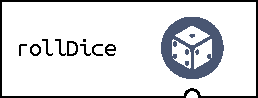
\includegraphics[scale=\scaling]{../illustrations/rollDice.pdf}
\end{center}
Εικόνα: Η συνάρτηση \pyinline{rollDice} είναι ένα ανεξάρτητο τμήμα κώδικα, ένα αυτόνομο ``εξάρτημα'' που επιτελεί μια συγκεκριμένη λειτουργία.}

\begin{pynew}
def rollDice():
    print("Ρίξε τα ζάρια πατώντας το ENTER...")
    input()
    dice1 = random.randint(1,6)
    dice2 = random.randint(1,6)
    roll = dice1 + dice2
    print("Έριξες", dice1, "και", dice2, "=", roll)
    return roll
\end{pynew}

Με τον τρόπο αυτό \emph{ορίζεται} η συνάρτηση \pyinline{rollDice()}, οι εντολές τις οποίας υλοποιούν το ``ρίξιμο'' των ζαριών.
Σημειώστε πως το αποτέλεσμα της συνάρτησης, δηλαδή η τιμή της μεταβλητής \pyinline{roll}, \emph{επιστρέφεται} από την συνάρτηση με την εντολή \pyinline{return}.
\end{step}

\begin{step}
Η συνάρτηση \pyinline{rollDice()} είναι σαν ένα μικρό ``εξάρτημα'' που επιτελεί μια συγκεκριμένη λειτουργία. Ωστόσο, αν και την κατασκευάσαμε, δεν την χρησιμοποιούμε πουθενά προς το παρόν.

Στο κύριο πρόγραμμα, στο σημείο όπου ρίχνονται για πρώτη φορά τα ζάρια, \emph{διαγράψτε} τις εντολές του βήματος~\ref{step:roll-commands}, που σχετίζονται με τη ρίψη των ζαριών και \emph{αντικαταστήστε} τις με τη γραμμή:
% [comment][removed] ώστε η ρίψη των ζαριών να πραγματοποιείται μέσω της συνάρτησης \pyinline{rollDice()} και η τιμή της ζαριάς να είναι η τιμή που επιστρέφεται από την συνάρτηση.

\begin{pynew}
roll = rollDice()
\end{pynew}

Με τη γραμμή αυτή ενεργοποιούμε ή \emph{καλούμε} την \pyinline{rollDice()}, πραγματοποιώντας έτσι τη ρίψη των ζαριών. Την τιμή που επιστρέφεται από την συνάρτηση, δηλαδή το άθροισμα των ζαριών, την ονομάζουμε \pyinline{roll}.

Εκτελέστε το πρόγραμμα. Λειτουργεί σωστά;

\marginnote[14pt]{\icondiscuss}
\dottedline

\marginnote[8pt]{\iconcaution}
Σε περίπτωση που κάτι πάει στραβά, βεβαιωθείτε ότι έχετε διαγράψει από το κύριο πρόγραμμα τις εντολές που αντιστοιχούν στο ρίξιμο της πρώτης ζαριάς, αφού αυτές εκτελούνται πλέον όταν καλείται το υποπρόγραμμα. Βεβαιωθείτε επίσης ότι η κλήση του υποπρογράμματος γίνεται στο κατάλληλο σημείο.

Παρατηρεί ο χρήστης κάποια διαφορά στη λειτουργία του προγράμματος, μετά από αυτή την τροποποίηση;

\marginnote[14pt]{\icondiscuss}
\dottedline
\end{step}

\begin{step}
\emph{Εντοπίστε} το σημείο του προγράμματος όπου ρίχνονται για δεύτερη φορά τα ζάρια. \emph{Διαγράψτε} τις σχετικές εντολές
%του βήματος~\ref{step:roll-commands}, 
που σχετίζονται με τη ρίψη των ζαριών και \emph{αντικαταστήστε} τις με μια ακόμα κλήση της συνάρτησης \pyinline{rollDice()}. 

\marginnote[18pt]{\iconcaution}
Φροντίστε να αποθηκεύσετε την τιμή που επιστρέφεται από την συνάρτηση στη μεταβλητή \pyinline{newroll}.

% [comment][changed] Δεν υπαγορεύουμε πλέον στα παιδιά πως θα γίνει η κλήση της συνάρτησης, πρέπει να το κάνουν μόνα τους.

%\begin{pynew}
%newroll = rollDice()
%\end{pynew}

% Εδώ καλούμε και πάλι την \pyinline{rollDice()}. 
% Την τιμή που επιστρέφεται από την συνάρτηση την ονομάζουμε \pyinline{newroll}.

\clearpage
Εκτελέστε το πρόγραμμα. Λειτουργεί σωστά;

\marginnote[14pt]{\icondiscuss}
\dottedline

Τι πιστεύετε ότι κερδίζουμε με την αντικατάσταση των αρχικών εντολών από την κλήση της συνάρτησης \pyinline{rollDice()};

\marginnote[14pt]{\icondiscuss}
\dottedline

\dottedline
\end{step}

% [comment] Από Βασίλη: Υπάρχουν άλλα σημεία του προγράμματος που θα προτείνατε να υλοποιηθούν ως υποπρόγραμμα; Αν ναι, ποια; Αν όχι, γιατί;

% [comment] Μέχρι εδώ δεν έχει ειπωθεί τίποτα για την επανάληψη. Θα μπορούσαμε να διακόψουμε, να ακολουθήσουμε ένα άλλο φύλλο εργασίας (π.χ. το πρώτο κομμάτι του guess) και μετά να επανέλθουμε.

\section{Τελική Εκδοχή}

Στη σημείο αυτό, ο κώδικας του κύριου προγράμματος, μετά τον ορισμό της \pyinline{rollDice()}, πρέπει να μοιάζει κάπως έτσι:

\begin{pyplain}
roll = rollDice()
if roll == 7 or roll == 11:
    print("Κέρδισες με την πρώτη!")
elif roll <= 3 or roll == 12:
    print("Έχασες με την πρώτη...") 
else:
    print("Ξαναρίξε. Πρέπει να φέρεις", roll)
    newroll = rollDice()
    if newroll == roll:
        print("Έφερες τη ζαριά-στόχο. Κέρδισες!")
    else:
        print("Έφερες διαφορετική ζαριά. Έχασες...")
\end{pyplain}

% [comment] Κάπου να γράψουμε ότι δεν είναι απαραίτητα ο καλύτερος τρόπος

Είμαστε κοντά στην τελική εκδοχή του παιχνιδιού. Στην πραγματικότητα, αν ο παίκτης δεν κερδίσει ούτε χάσει με την πρώτη ζαριά, τότε δεν ξαναρίχνει τα ζάρια μόνο μια φορά αλλά \emph{επαναληπτικά}, μέχρι να φέρει μια ζαριά ίση με την πρώτη του, οπότε κερδίζει. Αν όμως στο μεταξύ, φέρει \pyinline{7}, τότε χάνει.

%%%%%%%%%%%%%%%%%%%%%%%%%%%%%%%%%%%%%%%%%%%%%%%%%%%%%%%%%%%%%%%%%%%
% [comment] σημείο απόκλισης ανάμεσα στις δύο εκδοχές, με και χωρίς την break

\begin{step}
Στο ξεκίνημα της τρίτης περίπτωσης, όταν δηλαδή το παιχνίδι δεν έχει λήξει από την πρώτη ζαριά, %ο παίκτης καλείται να ρίξει και μια δεύτερη. Όμως οι κανόνες καθορίζουν ότι ίσως να χρειαστούν \emph{ακόμα περισσότερες} ζαριές, το πλήθος των οποίων δεν γνωρίζουμε εκ των προτέρων.
%Στο ξεκίνημα της τρίτης περίπτωσης, αμέσως μετά το \pyinline{else}, 
\emph{προσθέστε} ``μέσα'' στην \pyinline{else}:

\begin{pynew}
while True:
\end{pynew}

Προσθέστε \emph{τέσσερα κενά} μπροστά από όλες τις εντολές που ακολουθούν τη \pyinline{while}, σηματοδοτώντας έτσι ότι αυτές οι εντολές \emph{εμφωλεύονται} στη \pyinline{while}, δηλαδή περιέχονται σε αυτήν.

\marginnote[16pt]{\iconcaution}
Αν εκτελέσετε το πρόγραμμα και εμφανιστεί μήνυμα σφάλματος του τύπου \terminline{IndentationError: expected an indented block}, τότε ελέγξτε προσεκτικά τις \emph{εσοχές}. H \pyinline{while} πρέπει να βρίσκεται δεξιότερα της \pyinline{else} και οι εντολές που ακολουθούν ακόμα δεξιότερα.

\marginnote[22pt]{Mπορείτε να διακόψετε την εκτέλεση του προγράμματός σας με τον συνδυασμό πλήκτρων \terminline{Ctrl + C}.}
Εκτελέστε το πρόγραμμά σας. Αν κερδίσετε ή χάσετε με την πρώτη ζαριά τότε εκτελέστε το και πάλι. Ποια αλλαγή παρατηρείτε ότι επιφέρει η χρήση της \pyinline{while};

%\marginnote[14pt]{\icondiscuss}
\dottedline

%Υπάρχει κάτι που σας ενοχλεί; Κάτι που δεν δουλεύει σωστά;

%\marginnote[14pt]{\icondiscuss}
%\dottedline

%\marginnote[8pt]{\iconcaution}
%Σύμφωνα με τους κανόνες του παιχνιδιού, ο παίκτης θα πρέπει να ξαναρίξει τα ζάρια \emph{μόνο στην περίπτωση} που δεν κερδίσει και δεν χάσει με την πρώτη. Μήπως το πρόγραμμά σας του ζητά να τα ξαναρίξει ούτως ή άλλως;

%\marginnote[14pt]{\icondiscuss}
%\dottedline

%Αν όντως παρουσιάζεται αυτό το πρόβλημα, εξετάστε τις εσοχές που προηγούνται της \pyinline{while}. Μάλλον χρειάζεται να προσθέσετε περισσότερα κενά, για να υποδηλώσετε ότι ολόκληρη η \pyinline{while} βρίσκεται \emph{μέσα} στην \pyinline{else}, δηλαδή εκτελείται μόνο στην τρίτη περίπτωση.

% [comment] Προσθήκες από το φύλλο εργασίας του Βασίλη. Προς συζήτηση και επεξεργασία.
%Σε ποιο σημείο τοποθετήσατε την εντολή \pyinline{while}; Μέσα στην \pyinline{else} ή μετά από αυτή; Γιατί κάνατε αυτή την επιλογή;
%\marginnote[14pt]{\icondiscuss}
%\dottedline
%\dottedline

%Εκτελέστε το πρόγραμμά σας και βεβαιωθείτε ότι η επανάληψη εκτελείται μόνο στην περίπτωση που ο παίκτης δεν κερδίσει ή χάσει με την πρώτη και όχι σε κάθε περίπτωση.
\end{step}

\begin{step}
\emph{Τροποποιήστε} την \pyinline{if} που βρίσκεται μέσα στην επανάληψη. Η πρώτη περίπτωση δε χρειάζεται αλλαγή: ο παίκτης κερδίζει όταν φέρει την ίδια ζαριά με την αρχική. Ωστόσο, δεν χάνει σε οποιαδήποτε άλλη περίπτωση, αλλά μόνο όταν φέρει \pyinline{7}. 

\begin{pyplain}
        if newroll == roll:
            print("Έφερες τη ζαριά-στόχο. Κέρδισες!")
\end{pyplain}
\begin{pynew}
        elif |\textrm{\textit{συνθήκη}}|:   # συμπληρώστε την συνθήκη
            print("Έφερες 7. Έχασες...")
\end{pynew}

Παρατηρήστε ότι δεν υπάρχει πια η \pyinline{else}. Για ποιο λόγο πιστεύετε ότι συμβαίνει αυτό;

\marginnote[14pt]{\icondiscuss}
\dottedline

\dottedline

Εκτελέστε το πρόγραμμα. Υπάρχει κάτι που σας ενοχλεί; Κάτι που φαίνεται να μη δουλεύει σωστά;

\marginnote[14pt]{\icondiscuss}
\dottedline
\end{step}

\begin{step}
Η εντολή \pyinline{break} διακόπτει την επανάληψη μέσα στην οποία βρίσκεται αμέσως μόλις εκτελεστεί. \emph{Προσθέστε} την \pyinline{break} στο σημείο που θεωρείτε κατάλληλο, έτσι ώστε η επαναληπτική ρίψη των ζαριών να τερματίζεται όταν ο παίκτης ξαναφέρει την αρχική ζαριά--στόχο. 

Εκτελέστε το πρόγραμμα. Αν κερδίσετε ή χάσετε με την πρώτη ζαριά τότε εκτελέστε το και πάλι.
Σταματά η επανάληψη όταν ο παίκτης φέρει τη ζαριά--στόχο σε κάποια από τις επαναλαμβανόμενες ζαριές;

\marginnote[14pt]{\icondiscuss}
\dottedline

\begin{note}
Αν απαντήσατε αρνητικά, τότε βεβαιωθείτε ότι έχετε τοποθετήσει την \pyinline{break} μέσα στην αντίστοιχη περίπτωση της εμφωλευμένης \pyinline{if}.
\end{note}
\end{step}


\begin{step}
\emph{Προσθέστε} την \pyinline{break} στο σημείο που θεωρείτε κατάλληλο, έτσι ώστε η επαναληπτική ρίψη των ζαριών να τερματίζεται όταν ο παίκτης φέρει \pyinline{7}.

Εκτελέστε το πρόγραμμα. Σταματά η επανάληψη όταν ο παίκτης φέρει \pyinline{7} σε κάποια από τις επαναλαμβανόμενες ζαριές;

\marginnote[14pt]{\icondiscuss}
\dottedline
\end{step}

\section{Δραστηριότητες για Εξάσκηση}

\marginnote[16pt]{\href{http://pythonies.mysch.gr/complete/}{\url{pythonies.mysch.gr/complete}}}%
Για περισσότερη εξάσκηση στις έννοιες που γνωρίσατε σ' αυτό το φύλλο εργασίας, μπορείτε ν' ανατρέξετε στις ασκήσεις του %
Κεφαλαίου \href{http://pythonies.mysch.gr/chapters/craps.pdf}{``Μπαρμπούτι''}.

\end{document}




































%%%%%%%%%%%%%%%%%%%%%%%%%%%%%%%%%%%%%%%%%%%%%%%%%%%%%%%%%%%%%%%%%%%
% [comment] σημείο απόκλισης ανάμεσα στις δύο εκδοχές, με και χωρίς την break

\begin{step}
Στην τρίτη περίπτωση (``μέσα'' στο \pyinline{else}), όταν δηλαδή το παιχνίδι δεν έχει λήξει από την πρώτη ζαριά, ο παίκτης καλείται να ρίξει και μια δεύτερη. Όμως οι κανόνες καθορίζουν ότι ίσως να χρειαστούν \emph{ακόμα περισσότερες} ζαριές, το πλήθος των οποίων δεν γνωρίζουμε εκ των προτέρων.

\emph{Προσθέστε} τις εντολές που ακολουθούν, αμέσως μετά τη δεύτερη ζαριά του παίκτη και πριν την \pyinline{if} που ελέγχει το αποτέλεσμά της.

\begin{pynew}
    while True:
        print("Συνέχισε. Ο στόχος είναι το", roll)
        newroll = rollDice()
\end{pynew}

\marginnote[32pt]{\iconcaution}
Βεβαιωθείτε ότι έχετε κάνει σωστή χρήστη των \emph{εσοχών}, ώστε η \pyinline{while} να %βρίσκεται ``μέσα'' στην \pyinline{else} και να
εκτελείται \emph{μόνο} στην περίπτωση που το παιχνίδι δεν λήγει με την πρώτη ζαριά.

\marginnote[22pt]{Mπορείτε να διακόψετε την εκτέλεση του προγράμματός σας με τον συνδυασμό πλήκτρων \terminline{Ctrl + C}.}
Εκτελέστε το πρόγραμμα. Αν κερδίσετε ή χάσετε με την πρώτη ζαριά, εκτελέστε το και πάλι. Ποια αλλαγή παρατηρείτε ότι επιφέρει η χρήση της \pyinline{while};

%\marginnote[14pt]{\icondiscuss}
\dottedline

Τί πρόβλημα εντοπίζετε στη συμπεριφορά του προγράμματος, όπως έχει αυτή την στιγμή;

\marginnote[14pt]{\icondiscuss}
\dottedline

\dottedline

H \pyinline{while} ακολουθείται από μια \pyinline{if}. Πότε θα εκτελεστεί αυτή η \pyinline{if}; Να δικαιολογήσετε την απάντησή σας.

\marginnote[14pt]{\icondiscuss}
\dottedline

Τι \emph{πιστεύετε} ότι θα συνέβαινε αν τοποθετούσαμε τέσσερα κενά μπροστά από αυτή την \pyinline{if} και όλες τις εντολές που την ακολουθούν;

\marginnote[14pt]{\icondiscuss}
\dottedline

\dottedline

%Αν πιστεύετε ότι αυτή η αλλαγή είναι σωστή, πραγματοποιήστε την κι εκτελέστε το πρόγραμμα για να ελέγξετε την συμπεριφορά του. Διαφορετικά, αφήστε το πρόγραμμα ως έχει.
\end{step}

\begin{step}
Η \pyinline{while} συνοδεύεται από μια συνθήκη που ελέγχεται πριν από κάθε κύκλο της επανάληψης. Αν η συνθήκη είναι ψευδής (\pyinline{False}), τότε η επανάληψη σταματά. Όμως η τετριμμένη συνθήκη \pyinline{True} είναι πάντα αληθής, γι' αυτό η επανάληψη δεν σταματά ποτέ.

% [comment] Βασίλης: Προτείνω να τους δώσουμε τη while με την πρώτη συνθήκη και στη συνέχεια να γράψουν τη 2η συνθήκη χρησιμοποιώντας το AND.

Ποιά συνθήκη πρέπει να ελέγχεται από τη \pyinline{while}, έτσι ώστε η επανάληψη να συνεχίζεται όσο η ζαριά του χρήστη \emph{δεν} είναι ίδια με τη ζαριά στόχο;

\marginnote[14pt]{\icondiscuss}
\dottedline

\emph{Αντικαταστήστε} τη συνθήκη \pyinline{True} της \pyinline{while} με τη συνθήκη που απαντήσατε προηγουμένως. 

Εκτελέστε το πρόγραμμα. Σταματά η επανάληψη όταν ο παίκτης φέρει τη ζαριά--στόχο σε κάποια από τις επαναλαμβανόμενες ζαριές;

\marginnote[14pt]{\icondiscuss}
\dottedline

% [comment] Πιστεύω ότι πρέπει να τους δείξουμε τη συνθήκη της while γιατί είναι η πρώτη φορά που τη χρησιμοποιούν.
%\begin{pyplain}
%while |\pyhighlight{newroll != roll}|:
%\end{pyplain}
\end{step}

\begin{step}
Ποιά συνθήκη πρέπει να ελέγχεται από τη \pyinline{while}, έτσι ώστε η επανάληψη να συνεχίζεται όσο η ζαριά του χρήστη \emph{δεν} είναι το \pyinline{7};

\marginnote[14pt]{\icondiscuss}
\dottedline

\emph{Προσθέστε} στη συνθήκη της \pyinline{while} τη συνθήκη που απαντήσατε προηγουμένως. Οι δύο συνθήκες πρέπει να είναι \emph{συζευγμένες}, δηλαδή να ισχύουν και οι δύο για να συνεχίζεται η επανάληψη, οπότε χρησιμοποιήστε μεταξύ τους τον τελεστή \pyinline{and}.

Εκτελέστε το πρόγραμμα. Σταματά η επανάληψη όταν ο παίκτης φέρει~\pyinline{7} σε κάποια από τις επαναλαμβανόμενες ζαριές;

\marginnote[14pt]{\icondiscuss}
\dottedline

%Οι επαναληπτικές ρίψεις των ζαριών δεν πρέπει να σταματούν μόνο όταν ο παίκτης πετύχει τη ζαριά-στόχο, αλλά κι όταν ο παίκτης φέρει~\pyinline{7}. 

%\emph{Συμπληρώστε} τη συνθήκη της \pyinline{while} με μια πρόσθετη συνθήκη, έτσι ώστε η επανάληψη να συνεχίζεται επίσης όσο η ζαριά του χρήστη δεν ισούται με το~\pyinline{7}. 

%\marginnote[16pt]{\iconcaution}
%Οι δύο συνθήκες που θα ελέγχονται από τη \pyinline{while} πρέπει να είναι \emph{συζευγμένες} ή \emph{διαζευγμένες}; Πρέπει να ισχύουν και οι δύο για να συνεχιστεί η επανάληψη ή αρκεί να ισχύει μία από τις δύο; Στην πρώτη περίπτωση, χρησιμοποιήστε ανάμεσά τους τον τελεστή \pyinline{and}, ενώ στη δεύτερη τον τελεστή \pyinline{or}.
\end{step}

% [comment] Κι όταν προσθέσουμε την συνθήκη newroll != roll μπορούμε να ρωτήσουμε πότε θα εκτελεστεί η else της if, κλπ.

\begin{step}
Η \pyinline{if} που ακολουθεί τη \pyinline{while} ενημερώνει το χρήστη για το αποτέλεσμα του παιχνιδιού. 

Ποια είναι \emph{συγκεκριμένα} η ζαριά που πρέπει να έχει φέρει ο παίκτης για να εκτελεστεί η \pyinline{print} που βρίσκεται μέσα στην \pyinline{else}, στην τελευταία γραμμή του προγράμματος;

\marginnote[14pt]{\icondiscuss}
\dottedline

Το μήνυμα που εμφανίζει αυτή η \pyinline{print} δεν ταιριάζει πια με τους τελικούς κανόνες του παιχνιδιού. Να τροποποιήσετε την αντίστοιχη \pyinline{print}, ώστε να εμφανίζεται ένα κατάλληλο μήνυμα.\end{step}

